\section{Introduction}

\begin{definition}[\textit{Dependability}]
    Dependability is a measure of how much we trust a system. 
\end{definition}
Dependability can also be construed as the system's capacity to execute its intended functions while embodying:
\begin{itemize}
    \item \textit{Reliability}: the continuity of accurate service.
    \item \textit{Availability}: the readiness for accurate service.
    \item \textit{Maintainability}: the ease of maintenance.
    \item \textit{Safety}: the absence of catastrophic consequences.
    \item \textit{Security}: the preservation of data confidentiality and integrity.
\end{itemize}

Significant efforts are often directed towards functional verification, ensuring that the implementation aligns with specifications, fulfills requirements, meets constraints, and optimizes selected parameters.
However, even when all these aspects are addressed, system failures may still occur. 
Such failures are typically attributable to some form of breakdown.
\begin{figure}[H]
    \centering
    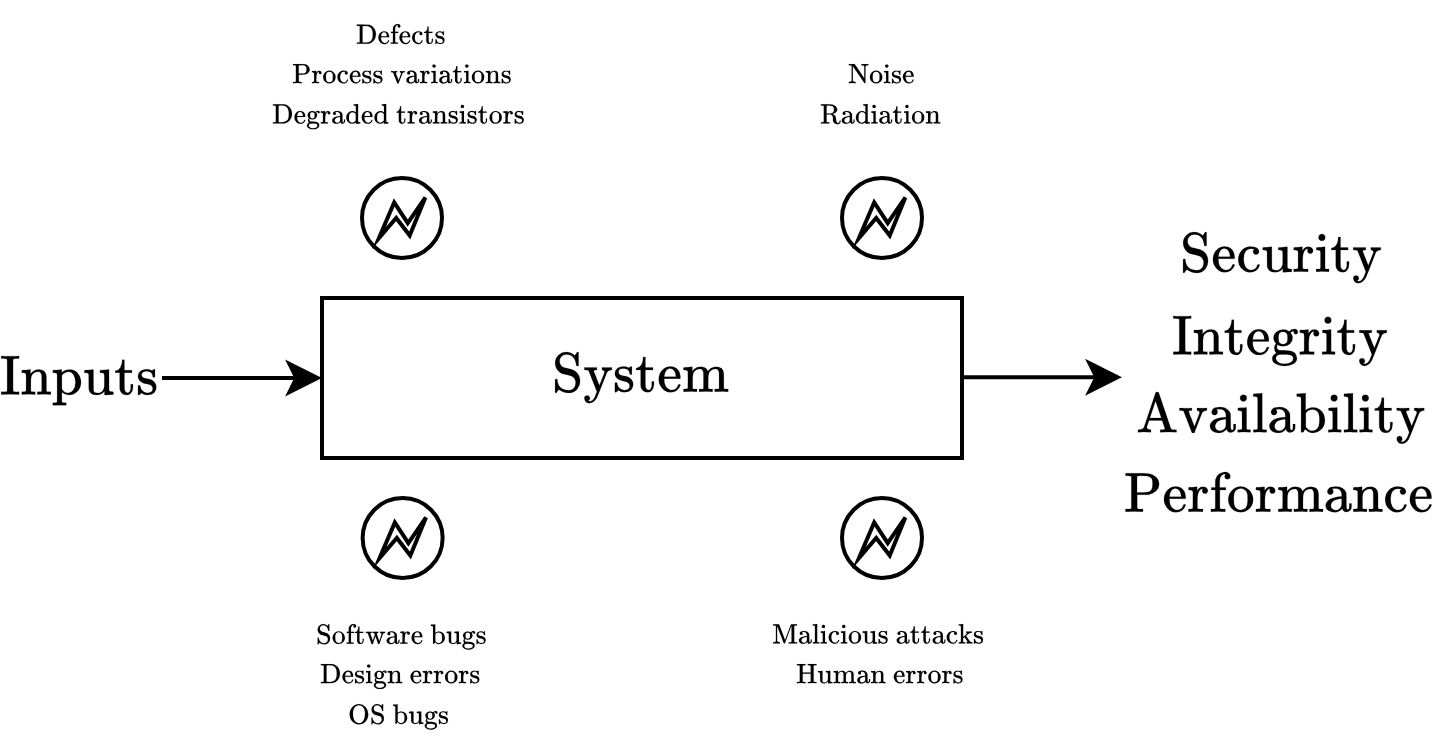
\includegraphics[width=0.5\linewidth]{images/dep.png}
    \caption{Dependability}
\end{figure}
A single system failure has the potential to impact a significant number of individuals.
The costs associated with a failure can be substantial, particularly if it results in economic losses or physical damage. 
Systems lacking in dependability are less likely to be utilized or embraced. 
Moreover, undependable systems can lead to information loss, incurring significant recovery costs.

To address these issues, specific standards have been established for various systems:
\begin{itemize}
    \item ISO 26262 for automotive.
    \item CENELEC 50128 (software) and 50129 (hardware) for railways.
    \item RTCA DO-178C (software) and DO-254 (hardware) for airborne systems.
    \item ESA ECSS-E-ST-40C (software) and ECSS-Q-ST-60-02C (hardware) for space systems.
\end{itemize}